% [原文 p.34]

\section{KZ 方程}
\takeaway{把点构形空间上的共形块空间拼成向量丛 $\cE_\lambda$，用 Sugawara 构造中的分量 $L_{-1}$ 定义其上的 KZ 联络；该联络平坦，水平截面的限制满足 KZ 方程，并在 Möbius 变换下按共形权作协变。}

Riemann 球面 $\CP^1$ 上 $n$ 个相异点的构形空间（configuration space）记作 $\Conf_n(\CP^1)$，即
\[
\Conf_n(\CP^1)=\{(p_1,\dots,p_n)\in(\CP^1)^n\mid \text{若 } i\ne j \text{ 则 } p_i\ne p_j\}.
\]
这里 $(\CP^1)^n$ 表示 $\CP^1$ 的 $n$ 重直积。上一节对 $p=(p_1,\dots,p_n)\in\Conf_n(\CP^1)$ 与 level $k$ 的最高权组 $\lambda=(\lambda_1,\dots,\lambda_n)$ 定义了共形块空间 $\cH(p,\lambda)$。本节让 $(p_1,\dots,p_n)$ 变动，把
\[
\cE_\lambda=\bigcup_{p\in\Conf_n(\CP^1)}\cH(p,\lambda)
\]
看作 $\Conf_n(\CP^1)$ 上的向量丛，在其上引入自然联络，并证明该联络的曲率为 $0$。

% [Tutor Note: 这个并集只用来指明纤维是 $\cH(p,\lambda)$，它本身还没有丛结构；真正的丛结构由下文把 $\cE_\lambda$ 嵌入平凡丛 $\Conf_n(\CP^1)\times\Hom_\C(\bigotimes_j\cH_{\lambda_j},\C)$ 来定义，不要把它当成简单的拓扑并集。]

取 $\CP^1$ 的 $n+1$ 重直积 $(\CP^1)^{n+1}$，令
\[
\pi:(\CP^1)^{n+1}\longrightarrow(\CP^1)^n
\]
为到前 $n$ 个分量的投影。用 $(z_1,\dots,z_n,z_{n+1})$ 表示 $(\CP^1)^{n+1}$ 的坐标函数。又记 $z_{n+1}-z_j=0$，$1\le j\le n$ 所定义的 $(\CP^1)^{n+1}$ 的超平面为 $D_j$。再令 $t_j=z_{n+1}-z_j$。

在 $\CP^1$ 上取相异的 $n$ 个点 $p_1,\dots,p_n$，其坐标分别为 $z_1,\dots,z_n$。$\pi^{-1}(p_1,\dots,p_n)=\CP^1$ 与 $D_j$（$1\le j\le n$）的交点，关于坐标函数 $z_{n+1}$ 的坐标恰好是 $z_1,\dots,z_n$。也就是说，把投影 $\pi$ 限制到点构形空间 $\Conf_n(\CP^1)$ 上，它相应于上述 $D_j$（$1\le j\le n$）给出 $n$ 个截面 $s_j$，$1\le j\le n$。于是，对 $\Conf_n(\CP^1)$ 的每一点 $p=(p_1,\dots,p_n)$，都对应一族 $\CP^1$，其上载有 $n$ 个相异点 $p_1,\dots,p_n$。

先取以 $\Hom_\C(\bigotimes_{j=1}^n\cH_{\lambda_j},\C)$ 为纤维、底为 $\Conf_n(\CP^1)$ 的平凡向量丛作为出发点；再在其内部构造一个子向量丛 $\cE_\lambda$，以共形块空间为纤维。直积 $\Conf_n(\CP^1)\times\Hom_\C(\bigotimes_{j=1}^n\cH_{\lambda_j},\C)$ 的元素 $(\bm{p},\Psi)$ 属于 $\cE_\lambda$，定义为 $\Psi$ 按上一节的意义是共形块空间的元素。

% [原文 p.35]

对 $\Conf_n(\CP^1)$ 的开集 $U$，$\cE_\lambda$ 在 $U$ 上的截面空间 $\Gamma(U,\cE_\lambda)$ 可描述如下。取一族以点 $\bm{p}\in U$ 为参数的多重线性映射
\[
\Psi(\bm{p}):\cH_{\lambda_1}\otimes\cdots\otimes\cH_{\lambda_n}\longrightarrow\C .
\]
以下设 $\bm{p}$ 的坐标为 $(z_1,\dots,z_n)$，并设 $\Psi(\bm{p})$ 关于 $z_1,\dots,z_n$ 可微。设 $f$ 为 $\pi^{-1}(U)$ 上取值于 Lie 代数 $\fg$ 的亚纯函数，极点至多在 $D_1,\dots,D_n$ 上。把亚纯函数 $f$ 沿 $D_j$（$1\le j\le n$）的 Laurent 展开写作
\[
f_{D_j}(t_j)=\sum_{m=-N}^{\infty}a_m(z_1,\dots,z_n)t_j^m .
\]
上式把 $f_{D_j}(t_j)$ 看作以 $z_1,\dots,z_n$ 的全纯函数为系数、关于 $t_j$ 的 Laurent 级数。与上一节共形块的定义相同，固定 $(z_1,\dots,z_n)$ 后，把 $f_{D_j}$ 看作仿射 Lie 代数 $\hat{\fg}_j=[\fg\otimes\C((t_j))]\oplus\C c$ 的元素。由此可以定义 Laurent 级数 $f_{D_j}(t_j)$ 在表示空间 $\cH_{\lambda_j}$ 上的作用。所谓 $\Psi$ 是开集 $U$ 上 $\cE_\lambda$ 的截面，是指：对 $\pi^{-1}(U)$ 上取值于 $\fg$、极点至多在 $D_1,\dots,D_n$ 的任意亚纯函数 $f$，以及 $\xi_j\in\cH_{\lambda_j}$（$1\le j\le n$），都有
\[
\sum_{j=1}^{n}[\Psi(\bm{p})](\xi_1,\dots,f_{D_j}\xi_j,\dots,\xi_n)=0
\]
对一切 $\bm{p}\in U$ 成立。特别地，固定 $\bm{p}$ 后，$\Psi(\bm{p})$ 是共形块空间 $\cH(\bm{p},\lambda)$ 的元素。由此可知 $\cE_\lambda$ 自然具有 $\Conf_n(\CP^1)$ 上向量丛的结构，称它为共形块丛。

以下利用 1.2 节 (1.9) 中由 Sugawara 算子引入的 Virasoro 算子 $L_{-1}$，在 $\Conf_n(\CP^1)$ 的子集
\[
\Conf_n(\C)=\{(z_1,\dots,z_n)\in\C^n\mid \text{若 } i\ne j \text{ 则 } z_i\ne z_j\}
\]
上描述向量丛 $\cE_\lambda$ 中的平坦联络。对仿射 Lie 代数 $\hat{\fg}$ 或其包络代数的元素 $X$，多重线性映射 $X^{(j)}\Psi:\cH_{\lambda_1}\otimes\cdots\otimes\cH_{\lambda_n}\to\C$ 由
\[
[X^{(j)}\Psi](\xi_1,\dots,\xi_n)=\Psi(\xi_1,\dots,X\xi_j,\dots,\xi_n),\qquad
\xi_1\in\cH_{\lambda_1},\ \dots,\ \xi_n\in\cH_{\lambda_n}
\]
定义；这里 $X$ 只作用在第 $j$ 个分量上。用这个记号可以证明下述命题。

% [原文 p.36]

\begin{proposition*}{1.16}
  设 $\Psi$ 是向量丛 $\cE_\lambda$ 在 $\Conf_n(\C)$ 上的截面，则
  \[
  \frac{\partial\Psi}{\partial z_j}-L_{-1}^{(j)}\Psi
  \]
  仍是 $\cE_\lambda$ 的截面。
\end{proposition*}

\begin{proof}
  对 $\Conf_n(\C)$ 的开集 $U$，取 $\pi^{-1}(U)$ 上取值于 $\fg$、极点至多在 $D_1,\dots,D_n$ 的亚纯函数 $f$，并把 $f$ 沿 $D_j$（$1\le j\le n$）的 Laurent 展开写作
  \[
  f_{D_j}(t_j)=\sum_{m=-N}^{\infty}a_m(z_1,\dots,z_n)t_j^m .
  \]
  偏导函数 $g=\dfrac{\partial f}{\partial z_j}$ 沿 $D_j$ 的 Laurent 展开，因 $t_j=z_{n+1}-z_j$，可写成
  \[
  \frac{\partial f}{\partial z_j}
  =\sum_{m=-N}^{\infty}\left(\frac{\partial a_m}{\partial z_j}t_j^{m}-a_m m\,t_j^{m-1}\right).
  \]
  把右端看作以 $z_1,\dots,z_n$ 的全纯函数为系数、关于 $t_j$ 的 Laurent 级数，记作 $g_{D_j}(t_j)$，则也可写成
  \[
  g_{D_j}(t_j)=\frac{\partial}{\partial z_j}f_{D_j}(t_j)-\frac{\partial}{\partial t_j}f_{D_j}(t_j).
  \]
  再由命题 1.6，
  \[
  \frac{\partial}{\partial t_j}f_{D_j}=-[L_{-1},f_{D_j}],
  \]
  因此
  \begin{equation}
    g_{D_j}=\frac{\partial}{\partial z_j}f_{D_j}+[L_{-1},f_{D_j}] \tag{1.20}
  \end{equation}
  成立。

% [原文 p.37]

把多重线性映射 $\Psi(\bm{p}):\cH_{\lambda_1}\otimes\cdots\otimes\cH_{\lambda_n}\to\C$ 简记为 $\Psi$，由上式得
\begin{equation}
\begin{aligned}
&\frac{\partial}{\partial z_j}\bigl[\Psi(\xi_1,\dots,f_{D_i}\xi_i,\dots,\xi_n)\bigr]\\
&\quad=\left(\frac{\partial\Psi}{\partial z_j}\right)(\xi_1,\dots,f_{D_i}\xi_i,\dots,\xi_n)
+\Psi\left(\xi_1,\dots,\frac{\partial}{\partial z_j}f_{D_i}\xi_i,\dots,\xi_n\right)
\end{aligned}
\tag{1.21}
\end{equation}
把此式与 (1.20) 合并，并利用 $\Psi$ 是共形块的元素这一事实，得到
\begin{align*}
&\sum_{i=1}^{n}\left(\frac{\partial\Psi}{\partial z_j}-L_{-1}^{(j)}\Psi\right)(\xi_1,\dots,f_{D_i}\xi_i,\dots,\xi_n)\\
&\quad=\sum_{i=1}^{n}\left\{\frac{\partial}{\partial z_j}\bigl[\Psi(\xi_1,\dots,f_{D_i}\xi_i,\dots,\xi_n)\bigr]
-\Psi(\xi_1,\dots,g_{D_i}\xi_i,\dots,\xi_n)\right\}.
\end{align*}
% [Tutor Note: 原书 p.37 此式左边求和对 $i$ 进行，而 $\Psi$ 中插入的是 $f_{D_i}\xi_i$，$L_{-1}$ 的上标却是 $(j)$，两处指标不一致；按下一行以 $g_{D_j}=\partial_{z_j}f_{D_j}+[L_{-1},f_{D_j}]$ 相消的推导，应以同一指标 $j$ 为准。此处照原书排印，存疑待考。]
注意 $\dfrac{\partial f}{\partial z_j}$ 也是极点至多在 $D_1,\dots,D_n$ 的亚纯函数，于是此式右端为 $0$，所要的结论得证。
\end{proof}

由这个命题，对向量丛 $\cE_\lambda$ 在 $\Conf_n(\C)$ 上的截面 $\Psi$，令
\begin{equation}
\nabla\Psi=\rd\Psi-\sum_{i=1}^{n}L_{-1}^{(i)}\Psi\,\rd z_i \tag{1.22}
\end{equation}
则 $\nabla$ 给出向量丛 $\cE_\lambda$ 的联络。此外，
\[
\omega=\sum_{i=1}^{n}L_{-1}^{(i)}\rd z_i
\]
满足 $\rd\omega=0$；又由
\[
[L_{-1}^{(i)},L_{-1}^{(j)}]=0,\qquad 1\le i,j\le n
\]
可得 $\omega\wedge\omega=0$。因此 $\nabla$ 的曲率为 $0$，即 $\nabla$ 是平坦联络（flat connection）。

% [Tutor Note: 这里把联络写成 $\nabla=\rd-\omega$，$\omega$ 取值于 $\End$；曲率为 $\rd\omega-\omega\wedge\omega$。由于 $L_{-1}^{(i)}$ 与 $L_{-1}^{(j)}$ 作用在不同分量上，二者交换，$\omega\wedge\omega=0$ 是显然的，真正要算的是 $\rd\omega=0$，即 $L_{-1}^{(i)}$ 不显含 $z$。]

其次，把 $\Psi:\cH_{\lambda_1}\otimes\cdots\otimes\cH_{\lambda_n}\to\C$ 限制到 $V_{\lambda_1}\otimes\cdots\otimes V_{\lambda_n}$，得到
\[
\Psi_0:V_{\lambda_1}\otimes\cdots\otimes V_{\lambda_n}\longrightarrow\C .
\]
下面把上述联络具体写出。先准备若干记号：取 Lie 代数 $\fg$ 的一组标准正交基 $\{I_\mu\}$，正交性由 Cartan--Killing 型给出，并令

% [原文 p.38]

\[
\Omega=\sum_{\mu}I_\mu\otimes I_\mu .
\]
又对 $i\ne j$（$1\le i,j\le n$），用 $\Omega^{(ij)}\Psi_0$ 表示 $\Omega$ 作用在 $\Psi_0$ 的第 $i$ 个与第 $j$ 个分量上。也就是说，对 $\xi_j\in V_{\lambda_j}$（$1\le j\le n$），令
\[
[\Omega^{(ij)}\Psi_0](\xi_1,\dots,\xi_n)
=\sum_{\mu}\Psi_0(\xi_1,\dots,I_\mu\xi_i,\dots,I_\mu\xi_j,\dots,\xi_n).
\]
由式 (1.15)，对 $X\otimes t^{-1}\in\hat{\fg}$ 与 $\xi_j\in V_{\lambda_j}$（$1\le j\le n$），有
\begin{equation}
\begin{aligned}
&\bigl[(X\otimes t^{-1})^{(i)}\Psi\bigr](\xi_1,\dots,\xi_n)\\
&\quad=\sum_{j,\,j\ne i}(z_i-z_j)^{-1}\Psi_0(\xi_1,\dots,X\xi_j,\dots,\xi_n)
\end{aligned}
\tag{1.23}
\end{equation}
而 Virasoro 算子 $L_{-1}$ 在表示空间 $V_{\lambda_j}$ 上的作用可写作
\[
L_{-1}=\frac{1}{k+2}\sum_{\mu}I_\mu\otimes t^{-1}\cdot I_\mu ,
\]
所以可以把 $\Psi$ 上的作用 $L_{-1}^{(i)}\Psi$ 限制到 $V_{\lambda_1}\otimes\cdots\otimes V_{\lambda_n}$ 来考虑。把它记作 $(L_{-1}^{(i)}\Psi)_0$。下述命题成立。

\begin{proposition*}{1.17}
  对共形块空间 $\cH(\bm{p},\lambda)$ 的元素 $\Psi$，$L_{-1}^{(i)}\Psi$ 在 $V_{\lambda_1}\otimes\cdots\otimes V_{\lambda_n}$ 上的限制 $(L_{-1}^{(i)}\Psi)_0$ 可表为
  \[
  (L_{-1}^{(i)}\Psi)_0=\frac{1}{k+2}\sum_{j,\,j\ne i}\frac{\Omega^{(ij)}\Psi_0}{z_i-z_j} .
  \]
  又，在同样的意义下，$L_{n}^{(i)}$（$n\ge 0$）的作用满足
  \begin{equation}
    (L_{n}^{(i)}\Psi)_0=0,\qquad n>0 \tag{1.24}
  \end{equation}
  \begin{equation}
    (L_{0}^{(i)}\Psi)_0=\Delta_{\lambda_i}\Psi_0 . \tag{1.25}
  \end{equation}
  这里 $\Delta_{\lambda_i}$ 是 $L_0$ 在不可约表示 $V_{\lambda_i}$ 上的作用的特征值。
\end{proposition*}

\begin{proof}
  关于 $L_{-1}$ 的作用，由式 (1.23)，

% [原文 p.39]

  \[
  \Psi(\xi_1,\dots,(I_\mu\otimes t^{-1}\cdot I_\mu)\xi_i,\dots,\xi_n)
  =\sum_{j,\,j\ne i}(z_i-z_j)^{-1}\Psi_0(\xi_1,\dots,I_\mu\xi_i,\dots,I_\mu\xi_j,\dots,\xi_n)
  \]
  成立，故所要的结果可得。关于 $L_n$（$n\ge 0$），看 $L_n$ 对 $\xi_i\in V_{\lambda_i}$ 的作用便知
  \[
  L_n\xi_i=0,\quad n>0;\qquad L_0\xi_i=\Delta_{\lambda_i}\xi_i ,
  \]
  由此立即得到结论。
\end{proof}

把命题 1.16 与命题 1.17 合起来可知：对向量丛 $\cE_\lambda$ 的联络 $\nabla$ 的水平截面（horizontal section），即满足 $\nabla\Psi=0$ 的截面 $\Psi$，将其限制到 $V_{\lambda_1}\otimes\cdots\otimes V_{\lambda_n}$ 所得的 $\Psi_0$ 满足微分方程
\[
\frac{\partial\Psi_0}{\partial z_i}=\frac{1}{k+2}\sum_{j,\,j\ne i}\frac{\Omega^{(ij)}\Psi_0}{z_i-z_j},
\qquad 1\le i\le n .
\]
这个微分方程称为 \textbf{Knizhnik--Zamolodchikov 方程}。以下常简称为 \textbf{KZ 方程}。此外，把 (1.22) 中引入的联络 $\nabla$ 称为 \textbf{KZ 联络}。

% [Tutor Note: KZ 方程右端的系数 $1/(k+2)$ 来自 Sugawara 构造中 $L_{-1}$ 的归一化 (1.9)；若改动 $L_n$ 的定义或 $c$ 的归一化，这个系数随之改变。核对文献时先看其 $L_{-1}$ 的写法，再比对系数。]

以下证明 KZ 联络的水平截面关于 Riemann 球面的 Möbius 变换具有某种协变性。下述命题用无穷小形式表述这一协变性。

\begin{proposition*}{1.18}
  设 $\Psi$ 是共形块丛 $\cE_\lambda$ 关于 KZ 联络 $\nabla$ 的水平截面，即满足 $\nabla\Psi=0$ 的截面，则其限制 $\Psi_0$ 在 $V_{\lambda_1}\otimes\cdots\otimes V_{\lambda_n}$ 上对 $r=-1,0,1$ 满足
  \[
  \sum_{i=1}^{n}z_i^{r}\left(z_i\frac{\partial}{\partial z_i}+(r+1)\Delta_{\lambda_i}\right)\Psi_0=0 .
  \]
\end{proposition*}

\begin{proof}
  首先，由命题中的 $\Psi_0$ 在 $\fg$ 的作用下不变可知
  \[
  \sum_{j=1}^{n}\Omega^{(ij)}\Psi_0=0,\qquad 1\le i\le n
  \]
  成立。由同样的理由，

% [原文 p.40]

  \[
  \sum_{i\ne j}\Omega^{(ij)}\Psi_0=-\sum_{j=1}^{n}\Omega^{(jj)}\Psi_0
  \]
  成立；又 $\Omega^{(ij)}$ 是 Casimir 算子，且具有对称性 $\Omega^{(ij)}=\Omega^{(ji)}$，故得
  \begin{equation}
    \sum_{1\le i<j\le n}\Omega^{(ij)}\Psi_0=-(k+2)\sum_{j=1}^{n}\Delta_{\lambda_j}\Psi_0 . \tag{1.26}
  \end{equation}
  当 $r=-1$ 时，
  \[
  \sum_{i=1}^{n}\frac{\partial\Psi_0}{\partial z_i}
  =\frac{1}{k+2}\sum_{i\ne j}\frac{\Omega^{(ij)}\Psi_0}{z_i-z_j},
  \]
  对此应用对称性 $\Omega^{(ij)}=\Omega^{(ji)}$，即得要证的结果。
  当 $r=0$ 时，
  \[
  \sum_{i=1}^{n}z_i\frac{\partial\Psi_0}{\partial z_i}
  =\frac{1}{k+2}\sum_{i\ne j}\frac{z_i\Omega^{(ij)}\Psi_0}{z_i-z_j},
  \]
  而
  \[
  \sum_{i\ne j}\frac{z_i\Omega^{(ij)}}{z_i-z_j}
  =\sum_{1\le i<j\le n}\Omega^{(ij)} ,
  \]
  与式 (1.26) 合并即得所要的结论。
  最后给出 $r=1$ 的情形。
  \[
  \sum_{i=1}^{n}z_i^{2}\frac{\partial\Psi_0}{\partial z_i}
  =\frac{1}{k+2}\sum_{i\ne j}\frac{z_i^{2}\Omega^{(ij)}\Psi_0}{z_i-z_j}
  \]
  的右端可变形为
  \[
  -\frac{2}{k+2}\left(\sum_{j=1}^{n}z_j\Omega^{(jj)}\right)\Psi_0 ,
  \]
  利用 $\Omega^{(ij)}$ 是 Casimir 算子即可完成证明。
\end{proof}

在上述命题中，$r=-1$ 的情形所得到的结果，意味着 $\Psi_0$ 关于平移
\[
w_j=z_j+c,\qquad c\in\C,\quad 1\le j\le n
\]

% [原文 p.41]

不变。又，$r=0$ 的情形表明 $\sum_{j=1}^{n}z_j\dfrac{\partial}{\partial z_j}$ 就是所谓的 Euler 算子，其结果是：$\Psi_0$ 关于相似变换
\[
w_j=\alpha z_j,\qquad \alpha\in\C,\quad 1\le j\le n
\]
按
\[
\Psi_0(w_1,\dots,w_n)=\alpha^{-\Delta_{\lambda_1}-\cdots-\Delta_{\lambda_n}}\Psi_0(z_1,\dots,z_n)
\]
变换。$r=1$ 时，考虑 Möbius 变换
\begin{equation}
  f_\varepsilon(z_j)=\frac{z_j}{-\varepsilon z_j+1} \tag{1.27}
\end{equation}
关于这个 Möbius 变换有
\[
\left.\frac{\rd}{\rd\varepsilon}\right|_{\varepsilon=0}\Psi_0(f_\varepsilon(z_1),\dots,f_\varepsilon(z_n))
=\sum_{j=1}^{n}z_j^{2}\frac{\partial}{\partial z_j}\Psi_0(z_1,\dots,z_n),
\]
故把命题中 $r=1$ 的情形写成积分形式，便得
\[
\Psi_0(f_\varepsilon(z_1),\dots,f_\varepsilon(z_n))
=\prod_{j=1}^{n}(-\varepsilon z_j+1)^{2\Delta_{\lambda_j}}\Psi_0(z_1,\dots,z_n).
\]
Riemann 球面 $\CP^1$ 的 Möbius 变换由平移、相似变换以及 (1.27) 型的一次分数变换生成，把这些合起来便得下述命题。

\begin{proposition}{1.19}
  对 Möbius 变换
  \[
  w_j=\frac{az_j+b}{cz_j+d},\qquad 1\le j\le n,
  \]
  \[
  a,b,c,d\in\C,\qquad ad-bc=1,
  \]
  $\Psi_0$ 满足
  \[
  \Psi_0(z_1,\dots,z_n)=\prod_{j=1}^{n}(cz_j+d)^{-2\Delta_{\lambda_j}}\Psi_0(w_1,\dots,w_n).
  \]
\end{proposition}

% [Tutor Note: 命题 1.19 把“新变量”写在右边：$\Psi_0(z)=\prod(cz_j+d)^{-2\Delta_j}\Psi_0(w)$，与 (1.29) 中 $\phi(v,f(z))=(f')^{-\Delta}\phi(v,z)$ 的方向一致；指数是 $2\Delta_{\lambda_j}$ 而不是 $\Delta_{\lambda_j}$，因为这里 $\Psi_0$ 有 $n$ 个协变分量、每个贡献一次权。]

这样一来，KZ 联络的水平截面关于 Möbius 变换的协变性就清楚了。借助这一协变性可知，KZ 联络可以在点构形空间 $\Conf_n(\CP^1)$ 整体上定义。

% [原文 p.42]

\section{顶点算子与算子积展开}
\takeaway{把共形块在三点 $0,p,\infty$ 上的取值读作作用子 $\phi(v,z)$，即顶点算子；它满足规范不变性 (1.28) 与共形协变性 (1.29)，而算子的交换关系完全由算子积展开（OPE）的奇异项决定。}

这里再次从场算子的立场来审视共形场理论。特别要说明顶点算子的表述方式，以及支配各种算子交换关系的算子积展开。

在 Riemann 球面 $\CP^1$ 上的三点 $0,p,\infty$ 处，分别给定 level $k$ 的最高权 $\lambda_0,\lambda,\lambda_\infty$，并按 1.4 节同样定义共形块空间。用 $z$ 表示点 $p$ 的坐标。共形块空间 $\cH(0,p,\infty;\lambda_0,\lambda,\lambda_\infty)$ 是线性映射
\[
\Psi:\cH_{\lambda_\infty}^{*}\otimes\cH_{\lambda}\otimes\cH_{\lambda_0}\longrightarrow\C
\]
的全体；这些映射至多以原点、无穷远点以及点 $p$ 为极点，并且关于取值于 $\fg$ 的亚纯函数在各点的 Laurent 展开所作的作用不变。把共形块空间的元素 $\Psi$ 限制到 $\cH_{\lambda_\infty}^{*}\otimes V_\lambda\otimes\cH_{\lambda_0}$，则关于 $X\otimes t^n$（$X\in\fg$）的作用的上述不变性，对 $u\otimes v\otimes w\in\cH_{\lambda_\infty}^{*}\otimes V_\lambda\otimes\cH_{\lambda_0}$ 可写成
\[
-\Psi((u(X\otimes t^n))\otimes v\otimes w)+z^{n}\Psi(u\otimes Xv\otimes w)
+\Psi(u\otimes v\otimes((X\otimes t^n)w))=0 .
\]
对满足此条件的 $\Psi$，令
\[
(\phi(v,z))(u\otimes w)=\Psi(u\otimes v\otimes w),
\]
则 $\phi(v,z)$ 关于 $v\in V_\lambda$ 线性，并给出依赖于 $z\in\C\setminus\{0\}$ 的双线性映射
\[
\phi(v,z):\cH_{\lambda_\infty}^{*}\otimes\cH_{\lambda_0}\longrightarrow\C .
\]
% [Tutor Note: 这里 $u$ 取自 $\cH_{\lambda_\infty}^{*}$ 而对偶空间的元素要做配对才落回 $\C$；把 $\phi(v,z)$ 读作“从 $\cH_{\lambda_0}$ 到 $\cH_{\lambda_\infty}$ 的算子”时，方向来自 $\cH^{*}$ 的自对偶与配对，不要误以为 $\Psi$ 的第三个因子 $\cH_{\lambda_0}$ 是作用的对象。]
把它看作从 $\cH_{\lambda_0}$ 到无限直积 $\bar{\cH}_{\lambda_\infty}=\prod_{d\ge 0}\cH_{\lambda_\infty,d}$ 的算子。于是，关于亚纯函数 $X\otimes t^n$ 的作用的不变性，可表成 $\phi(v,z)$ 与 $X\otimes t^n$（$X\in\fg$）的交换关系：
\begin{equation}
  [X\otimes t^n,\phi(v,z)]=z^{n}\phi(Xv,z) \tag{1.28}
\end{equation}
这称为规范不变性（gauge invariance）。进一步，把 $\Psi$ 在 $V_{\lambda_\infty}^{*}\otimes V_\lambda\otimes V_{\lambda_0}$ 上的限制 $\Psi_0$ 取作前一节导出的 KZ 联络的水平截面，则可以证明相应的 $\phi(v,z)$ 满足

% [原文 p.43]

\begin{equation}
  [L_n,\phi(v,z)]=z^{n}\left(z\frac{\rd}{\rd z}+(n+1)\Delta_\lambda\right)\phi(v,z). \tag{1.29}
\end{equation}
满足关系式 (1.28) 与 (1.29) 的算子称为\textbf{顶点算子}（chiral vertex operator），或称 \textbf{primary 场}（primary field）。

% [Tutor Note: (1.29) 中 $n$ 取遍整数，而 (1.24)、(1.25) 只对 $n\ge 0$ 陈述；两者说的是不同对象：前者是绕 $z$ 的围道积分给出的算子，后者是它在最高权表示顶端 $V_\lambda$ 上的分量。若把两处的 $n$ 混为一谈，会误以为负模作用为零。]

条件 (1.29) 可以解释为 $\phi(v,z)(\rd z)^{\Delta_\lambda}$ 关于全纯共形变换的不变性，理由如下。把 $w=f(z)$ 所描述的全纯变换下 $\phi(v,z)(\rd z)^{\Delta_\lambda}$ 的不变性写出，即为
\[
\phi(v,f(z))=\left(\frac{\rd f}{\rd z}\right)^{-\Delta_\lambda}\phi(v,z).
\]
考虑其无穷小形式，假设在共形变换 $f_\varepsilon(z)=z-\varepsilon(z)$ 下不变，则 $\phi(v,z)$ 经 $f_\varepsilon$ 的无穷小位移 $\delta_\varepsilon\phi(v,z)$ 形如
\[
\delta_\varepsilon\phi(v,z)=\left(\Delta_\lambda\varepsilon'(z)+\varepsilon(z)\frac{\partial}{\partial z}\right)\phi(v,z).
\]
特别地，取 $\varepsilon(z)=\varepsilon z^{n+1}$ 时，上式由条件 (1.29) 的右端给出。另一方面，变换 $f_\varepsilon=z-\varepsilon z^{n+1}$ 生成向量场 $-z^{n+1}\dfrac{\rd}{\rd z}$，故可认为它作为无穷小变换由条件 (1.29) 的左端给出。

对表示空间 $\cH_\lambda$ 定义算子 $X(z)$、$T(z)$（$X\in\fg$，$z\in\C\setminus\{0\}$）：
\begin{equation}
  X(z)=\sum_{n\in\Z}(X\otimes t^n)z^{-n-1} \tag{1.30}
\end{equation}
\begin{equation}
  T(z)=\sum_{n\in\Z}L_n z^{-n-2} \tag{1.31}
\end{equation}
$T(z)$ 称为能量-动量张量（energy momentum tensor）。

下面说明描述这些算子之合成的算子积展开（OPE）。在区域 $|w|>|z|>0$ 内，算子 $X(w)$ 与 $\phi(v,z)$ 的合成具有
\begin{equation}
  X(w)\phi(v,z)=\frac{1}{w-z}\phi(Xv,z)+\bigl((w-z)\text{ 的正则项}\bigr) \tag{1.32}
\end{equation}
形式的展开。

% [原文 p.44]

它在区域 $|z|>|w|>0$ 内解析延拓为 $\phi(v,z)X(w)$。算子的合成写成这样的表示，称为\textbf{算子积展开}（operator product expansion）。它描述算子 $X(w)$ 与 $\phi(v,z)$ 的合成在 $w=z$ 处具有怎样的奇性。算子积展开可以直接由交换关系 (1.28) 得出；但如下文所述，反过来，算子积展开才是规定算子交换关系的有力工具。在物理学家撰写的文献中，常常反过来以算子积展开为出发点来组织理论。

对 $T(z)$ 与 $\phi(v,z)$，在区域 $|w|>|z|>0$ 内同样有算子积展开
\begin{equation}
\begin{aligned}
T(w)\phi(v,z)&=\left(\frac{\Delta_\lambda}{(w-z)^{2}}+\frac{1}{w-z}\frac{\partial}{\partial z}\right)\phi(v,z)
+\bigl((w-z)\text{ 的正则项}\bigr)
\end{aligned}
\tag{1.33}
\end{equation}
成立。它在区域 $|z|>|w|>0$ 内解析延拓为 $\phi(v,z)T(w)$。

$T(z)$ 之间的合成也写出算子积展开。在区域 $|w|>|z|>0$ 内有展开
\begin{equation}
\begin{aligned}
T(w)T(z)&=\frac{c/2}{(w-z)^{4}}+\frac{2T(z)}{(w-z)^{2}}+\frac{1}{w-z}\frac{\partial}{\partial z}T(z)\\
&\quad+\bigl((w-z)\text{ 的正则项}\bigr)
\end{aligned}
\tag{1.34}
\end{equation}
成立，它在区域 $|z|>|w|>0$ 内解析延拓为 $T(z)T(w)$。

下面看如何由算子积展开重新得到算子的交换关系。

\begin{figure}[htbp]
  \centering
  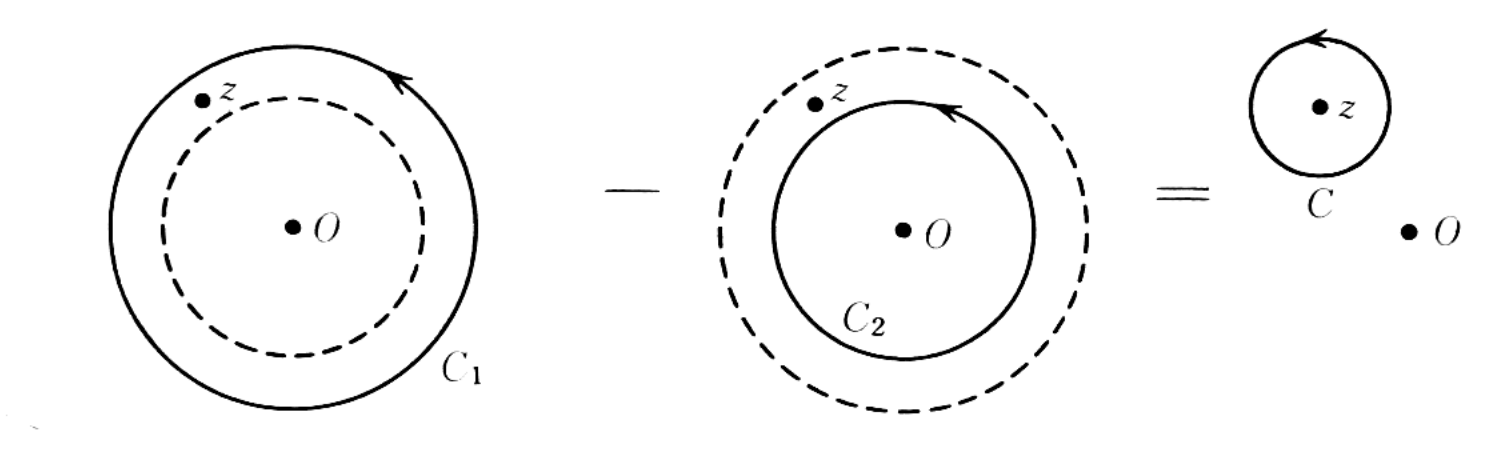
\includegraphics[width=0.78\textwidth]{figures/fig1.3.png}
  \figtitle{1.3}{积分路的变形与交换关系的解释（原书 p.44）}
\end{figure}

% [原文 p.45]

首先说明 $X\otimes t^n$ 以及 $L_n$ 与 $\phi(v,z)$ 的交换子可以表成
\begin{equation}
  [X\otimes t^n,\phi(v,z)]=\frac{1}{2\pi\sqrt{-1}}\int_{C}w^{n}X(w)\phi(v,z)\rd w \tag{1.35}
\end{equation}
\begin{equation}
  [L_n,\phi(v,z)]=\frac{1}{2\pi\sqrt{-1}}\int_{C}w^{n+1}T(w)\phi(v,z)\rd w \tag{1.36}
\end{equation}
这里积分路 $C$ 是 $w$ 平面上绕 $z$ 正向一周的充分小的圆周。事实上，$L_n\phi(v,z)$ 可写成
\[
\frac{1}{2\pi\sqrt{-1}}\int_{C_1}w^{n+1}T(w)\phi(v,z)\rd w ,
\]
其中 $C_1$ 是 $w$ 平面上满足 $|w|>|z|$、绕原点正向一周的圆周；而 $\phi(v,z)L_n$ 也可写成
\[
\frac{1}{2\pi\sqrt{-1}}\int_{C_2}w^{n+1}\phi(v,z)T(w)\rd w ,
\]
其中 $C_2$ 是 $w$ 平面上满足 $|z|>|w|$、绕原点正向一周的圆周。由于 $T(w)\phi(v,z)$（$|w|>|z|>0$）解析延拓为 $\phi(v,z)T(w)$（$|z|>|w|>0$），按图1.3 取积分路即得要证的结果。与算子积展开 (1.33) 比较可知，由此重新得到交换关系 (1.29)。由此可见，算子的交换关系由算子积展开所支配。因此，算子 $\phi(v,z)$ 关于全纯共形变换的协变性，可以看作算子积展开 (1.33) 的推论。对 $X\otimes t^n$ 一方同样可由算子积展开导出规范不变性。

% [Tutor Note: 图1.3 的实质是：先取满足 $|w|>|z|$ 的圆 $C_1$ 与满足 $|z|>|w|$ 的圆 $C_2$，两者之差等于绕 $z$ 的小圆 $C$；把 $L_n\phi$ 与 $\phi L_n$ 的围道积分相减，再用 (1.33) 的奇性项取留数，就得到 (1.29)。作者只写“取积分路”而省略了这一步留数计算。]

下面说明由算子积展开 (1.34) 可以导出 Virasoro 代数的交换关系。首先，设 $\gamma$ 为 $z$ 平面上绕原点正向一周的圆周，则 $L_n$ 可表为
\[
L_n=\frac{1}{2\pi\sqrt{-1}}\int_{\gamma}z^{n+1}T(z)\rd z .
\]
又，Sugawara 算子的合成 $L_mL_n$ 可如下表示：取 $w$ 平面上绕原点正向一周的圆周 $\gamma_1$ 与 $z$ 平面上绕原点正向一周的圆周 $\gamma_2$，使 $\gamma_1$ 的半径大于 $\gamma_2$ 的半径，则

% [原文 p.46]

\[
L_mL_n=\left(\frac{1}{2\pi\sqrt{-1}}\right)^{2}\int_{\gamma_1}\int_{\gamma_2}w^{m+1}z^{n+1}T(w)T(z)\rd w\,\rd z .
\]
对 $L_nL_m$ 也可在 $|z|>|w|$ 的情形作同样的描述。对它作解析延拓，并如图1.3 那样，在 $w$ 平面上取绕 $z$ 正向一周的曲线 $C$，计算积分
\[
\frac{1}{2\pi\sqrt{-1}}\int_{C}w^{m+1}z^{n+1}T(w)T(z)\rd w
\]
在 $z=0$ 处的留数。由此得到 $L_mL_n-L_nL_m$，命题 1.7 所述的 Sugawara 算子满足的 Virasoro 代数关系式便被重新得到。

为写出能量-动量张量 $T(z)$ 关于共形变换的变换法则，引入 \textbf{Schwarz 导数}（Schwarzian derivative）
\begin{equation}
  S(f,z)=\frac{f'''(z)}{f'(z)}-\frac{3}{2}\left(\frac{f''(z)}{f'(z)}\right)^{2}. \tag{1.37}
\end{equation}
众所周知，下述引理成立。

\begin{lemma}{1.20}
  对一次分数变换
  \[
  f(z)=\frac{az+b}{cz+d},\qquad a,b,c,d\in\C,\quad ad-bc=1,
  \]
  有 $S(f,z)=0$。反之，若 $S(f,z)=0$，则 $f$ 是一次分数变换。
\end{lemma}

% [Tutor Note: (1.37) 的系数 $3/2$ 是使 Schwarz 导数满足链式法则的唯一取法；若把它改掉，$S$ 就不再是共形不变量，(1.38) 的 $c/12$ 与 (1.34) 的 $c/2$ 也不能再与它配套。三处由同一个中心荷 $c$ 决定，改一处就必须同时改另外两处。]

与顶点算子的情形相同，用 $T(z)$ 的交换关系写出共形变换 $f_\varepsilon(z)=z-\varepsilon(z)$ 引起的无穷小位移 $\delta_\varepsilon T(z)$，可得
\begin{equation}
  \delta_\varepsilon T(z)=\varepsilon(z)\frac{\partial}{\partial z}T(z)+2\varepsilon'(z)T(z)+\frac{c}{12}\varepsilon'''(z). \tag{1.38}
\end{equation}
由于末项 $\dfrac{c}{12}\varepsilon'''(z)$ 存在，$T(z)$ 不是二阶共变张量。不过，若令 $\varepsilon(z)=\varepsilon z^{n+1}$，则仅当 $n=-1,0,1$，即 $L_n$ 生成一次分数变换时，这一项才为 $0$。因此，把 (1.38) 写成积分形式便得下述命题。

\begin{proposition}{1.21}
  能量-动量张量 $T(z)$ 在全纯变换 $w=f(z)$ 下，

% [原文 p.47]

  按
  \[
  T(z)=\left(\frac{\partial w}{\partial z}\right)^{2}T(w)+\frac{c}{12}S(f,z)
  \]
  变换。
\end{proposition}

% [Tutor Note: (1.38) 与命题 1.21 的对应要看清自变量：$T(z)$ 换成 $T(w)$ 时乘的是 $(\partial w/\partial z)^{2}$，而 Schwarz 导数 $S(f,z)$ 的第三个变元仍记作 $z$。若把 $\partial w/\partial z$ 误写成 $\partial z/\partial w$，中心荷项的符号会跟着出错。]

在上述讨论的基础上，概览环面的共形块空间。取 $\tau\in\C$ 为复上半平面的元素，令 $\Gamma$ 为由 $1$ 与 $\tau$ 在 $\Z$ 上生成的格 $\Z\oplus\Z\tau$。下面定义环面 $E=\C/\Gamma$ 的共形块空间。在复解析同构的范围内可设 $0\le\Re\tau<1$，故如此假设，并令 $q=\ee^{2\pi\ii\tau}$。让由相似变换 $f(w)=qw$ 生成的群 $G$ 作用在 $\C^{*}=\C\setminus\{0\}$ 上，考虑商空间 $\C^{*}/G$。在对应 $w=\ee^{2\pi\ii z}$ 之下，$\C^{*}/G$ 与环面 $E$ 同构；如图1.4 所示，$1$ 与 $\tau$ 张成的平行四边形在 $\C^{*}$ 中的像，是由 $|q|\le|w|\le 1$ 确定的圆环区域 $D$。环面由圆 $|w|=1$ 与 $|w|=|q|$ 经相似变换 $f(w)=qw$ 粘合而得。

\begin{figure}[htbp]
  \centering
  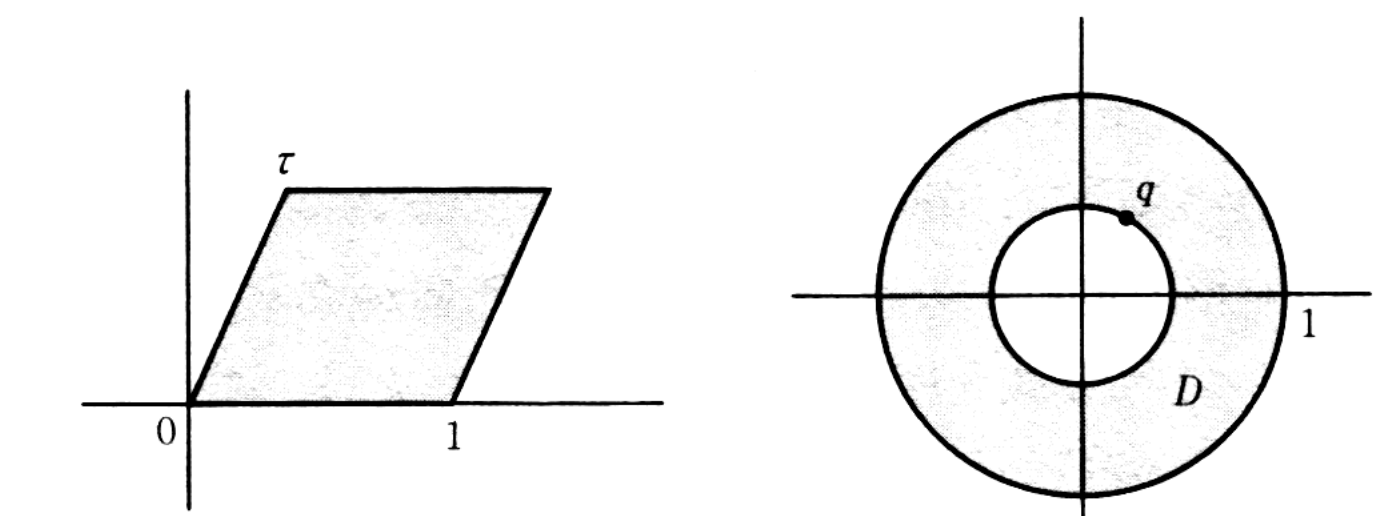
\includegraphics[width=0.72\textwidth]{figures/fig1.4.png}
  \figtitle{1.4}{环面的基本区域及其在变换 $w=\ee^{2\pi\ii z}$ 下的像（原书 p.47）}
\end{figure}

变换 $w=\ee^{2\pi\ii z}$ 把复平面移到 $\C^{*}$；计算该变换的 Schwarz 导数可知，$\C^{*}$ 一侧的 Virasoro 算子 $L'_0$ 可用原来的 $L_0$ 表为
\[
L'_0=L_0-\frac{c}{24}.
\]
又由此可知，相似变换 $f(w)=qw$ 在最高权表示 $\cH_\lambda$ 上的作用，关于 (1.11) 的谱分解 $\bigoplus_{d\ge 0}\cH_{\lambda,d}$，由

% [原文 p.48]

\begin{equation}
  q^{L_0-\frac{c}{24}}\xi
  =\exp\left(2\pi\sqrt{-1}\tau\left(\Delta_\lambda+d-\frac{c}{24}\right)\right)\xi,
  \qquad \xi\in\cH_{\lambda,d} \tag{1.39}
\end{equation}
给出。
在环面 $\C/\Gamma$ 上取相异点 $p_1,\dots,p_n$，并给这些点赋以 level $k$ 的最高权 $\mu_1,\dots,\mu_n$。把点 $p_1,\dots,p_n$ 表为区域 $D$ 的点。此外，在 $w$ 平面上，于原点处给定 level $k$ 的最高权 $\lambda$ 的对偶表示，于无穷远点处给定 level $k$ 的最高权 $\lambda$，并考虑与这些数据相应的 Riemann 球面的共形块空间。对其中元素 $\Phi$，把由 $f(w)=qw$ 确定的相似变换的作用 (1.39) 作用在原点与无穷远点对应的表示空间上，再约化张量积，所得映射记为
\[
\Tr_{\cH_\lambda}q^{L_0-\frac{c}{24}}\Phi:\cH_{\mu_1}\otimes\cdots\otimes\cH_{\mu_n}\longrightarrow\C ,
\]
再由这些映射生成线性空间 $\cH_\lambda(D)$。进一步令
\[
\cH_E(p,\mu)=\bigoplus_{\lambda}\cH_\lambda(D),
\]
称之为环面 $E$ 的共形块空间。这里，和取遍 level $k$ 的全部最高权 $\lambda=0,1,\dots,k$。

特别地，$n=0$ 时，可取
\begin{equation}
  \chi_\lambda(\tau)=\Tr_{\cH_\lambda}q^{L_0-\frac{c}{24}},\qquad
  \lambda=0,1,\dots,k \tag{1.40}
\end{equation}
作为共形块空间的基底。由式 (1.40) 定义的 $\chi_\lambda(\tau)$（$\lambda=0,1,\dots,k$）称为 $A_1^{(1)}$ 型仿射 Lie 代数的指标（character）。环面共形块空间的基底就这样由仿射 Lie 代数的指标给出，这些指标称为 Verlinde 基底。如文献 [8] 所述，Kac--Peterson 证明了：$A_1^{(1)}$ 型仿射 Lie 代数的指标关于 $SL_2(\Z)$ 的作用，按
\begin{equation}
\begin{aligned}
\chi_\lambda\left(-\frac{1}{\tau}\right)&=\sum_{\mu}S_{\lambda\mu}\chi_\mu(\tau),\\
\chi_\lambda(\tau+1)&=\exp\left(2\pi\sqrt{-1}\left(\Delta_\lambda-\frac{c}{24}\right)\right)\chi_\lambda(\tau)
\end{aligned}
\tag{1.41}
\end{equation}
变换。这里，$S_{\lambda\mu}$、$\Delta_\lambda$ 分别由

% [原文 p.49]

\begin{equation}
  S_{\lambda\mu}=\sqrt{\frac{2}{k+2}}\ \sin\frac{(\lambda+1)(\mu+1)\pi}{k+2} \tag{1.42}
\end{equation}
\begin{equation}
  \Delta_\lambda=\frac{\lambda(\lambda+2)}{4(k+2)} \tag{1.43}
\end{equation}
给出。$\Delta_\lambda$ 是 Sugawara 算子 $L_0$ 在 $V_\lambda$ 上的特征值，也就是前面称为共形权的量。这些量在后文的讨论中会反复出现。

% [Tutor Note: (1.40) 里 $q^{L_0-c/24}$ 的 $c$ 是 Virasoro 中心荷，与 level $k$ 的关系为 $c=3k/(k+2)$；(1.43) 的 $\Delta_\lambda=\lambda(\lambda+2)/(4(k+2))$ 正是从 Sugawara 构造的 $L_0$ 在 $V_\lambda$ 上的特征值算出来的。把 $\Delta_\lambda$ 当成自由参数会与 (1.42) 的 $S$ 矩阵对不上。]

下面说明 level $k$ 的 $SU(2)$ Wess--Zumino--Witten 模型的 Verlinde 代数。以 $v_\lambda$（$\lambda=0,1,\dots,k$）为基，取复线性空间 $R_k$，并用
\[
v_\lambda\cdot v_\mu=\sum_{\nu}N_{\lambda\mu}^{\nu}v_\nu
\]
在 $R_k$ 上引入积结构。这里 $N_{\lambda\mu}^{\nu}$ 取 $0$ 或 $1$，是命题 1.15 中所述的、给 Riemann 球面三点赋以 level $k$ 的最高权时共形块空间的维数。此处处理的是 $\fg=\fsl_2(\C)$ 的情形，故 $N_{\lambda\mu}^{\nu}=N_{\lambda\mu\nu}$。如 1.3 节所说明，用图1.2 的两种图计算给 Riemann 球面四点赋以 level $k$ 的最高权时的共形块空间，便可看出 $R_k$ 关于上述积满足结合律。$R_k$ 称为 Verlinde 代数，或融合代数（fusion algebra）。

设 $N_\lambda$ 为 $\mu\nu$ 分量等于 $N_{\lambda\mu\nu}$ 的 $k+1$ 阶方阵。特别地，$N_1$ 的 $ij$ 分量在 $|i-j|=1$ 时为 $1$、其余情形为 $0$；它被 (1.42) 的 $S=(S_{\lambda\mu})$ 对角化，特征值为 $S_{1\mu}/S_{0\mu}$（$\mu=0,1,\dots,k$）。可以验证 $N_\lambda$ 能写成 $N_1$ 的多项式，因此它同样被 $S$ 对角化，特征值为 $S_{\lambda\mu}/S_{0\mu}$（$\mu=0,1,\dots,k$）。由此可得下述命题。

\begin{proposition}{1.22}
  （Verlinde 等式）共形块空间的维数 $N_{\lambda\mu\nu}$ 可用矩阵 $S$ 表为
  \[
  N_{\lambda\mu\nu}=\sum_{\alpha}\frac{S_{\lambda\alpha}S_{\mu\alpha}S_{\nu\alpha}}{S_{0\alpha}} .
  \]
\end{proposition}

% [原文 p.50]

上述命题在代数上可以改述如下。在 $R_k$ 中，把基底作变换
\[
w_\mu=S_{0\mu}\sum_{\lambda}S_{\lambda\mu}v_\lambda ,
\]
便有
\[
w_\lambda\cdot w_\mu=\delta_{\lambda\mu}w_\lambda
\]
成立。也就是说，$w_\lambda$ 成为幂等元。Verlinde 原来的主张是：一般共形场理论的融合规则，可由模变换的 $S$ 矩阵对角化；这里所述的只是它的一个特殊情形。

% [Tutor Note: 命题 1.22 的右端以 $S_{0\alpha}$ 作分母，故 $\alpha$ 从 $0$ 取到 $k$；$\lambda,\mu,\nu$ 也同此范围。$N_{\lambda\mu\nu}$ 关于三个指标对称，这与 $R_k$ 的交换性一致，但 (1.22) 用的 $S$ 只对 $A_1^{(1)}$ 型给出 (1.42) 的显式公式，换其他型时 $S$ 要另行计算。]

\section*{小结}
\addcontentsline{toc}{section}{小结}
\markright{小结}

\textbf{1.1}\ 定义了环路代数的中心扩张，即仿射 Lie 代数；又定义了 $S^1$ 上多项式向量场构成的 Lie 代数的复化的中心扩张，即 Virasoro 代数。

\textbf{1.2}\ 证明了由描述环路代数中心扩张的 2-余循环，可以构造环路群上的复线丛。

\textbf{1.3}\ 证明了在 Wess--Zumino--Witten 模型中，对带边界的 Riemann 面 $\Sigma$，$\exp(-S_\Sigma(f))$ 可看作环路群上复线丛的纤维的元素。

\textbf{1.4}\ 定义了 Riemann 球面上共形块的空间，并叙述了给出其维数的融合规则。

\textbf{1.5}\ 构造了点构形空间上的共形块丛，并证明了该向量丛上自然存在称为 KZ 联络的平坦联络。

\textbf{1.6}\ 定义了顶点算子，并叙述了与之相关的算子积展开。

\chapterreview{%
第 1 章为全书准备语言。它把 Wess--Zumino--Witten 模型的共形块从“场论的配分函数”变成点构形空间上的向量丛及其水平截面，使第 2 章关于辫群表示、第 3 章关于微扰展开的讨论都有了可计算的载体；全书三次出现的“共形块——平坦联络——顶点算子”三角关系，也在这里定型。本章同时冻结了全书的记号：$\cH_\lambda$、$V_\lambda$、$\cE_\lambda$、$L_n$ 与常数 $1/(k+2)$ 的用法此后不再重复定义。

全章可分两层。§1.1--§1.3 是代数与场论的基础：环路群、仿射 Lie 代数及其中心扩张、最高权表示、WZW 作用量与复线丛，说明 $e^{-S}$ 作为线丛纤维元素的意义。§1.4--§1.6 转入几何：先用共形块与融合规则给出维数 $N_{\lambda\mu\nu}$，再构造共形块丛 $\cE_\lambda$ 与 KZ 联络，最后用顶点算子 $\phi(v,z)$ 与算子积展开把同一结构翻译成算子语言。共形块、平坦联络、顶点算子这三层对象，其实是同一件事的三种写法。

本章的核心结论有四条。其一，$\cE_\lambda$ 上有自然的平坦联络 (1.22)，其水平截面在 $V_{\lambda_1}\otimes\cdots\otimes V_{\lambda_n}$ 上的限制满足 KZ 方程，系数为 $1/(k+2)$。其二，水平截面关于 Möbius 变换按 (1.19) 协变，正是这一协变性保证 KZ 联络能从 $\Conf_n(\C)$ 整体地搬到 $\Conf_n(\CP^1)$ 上。其三，顶点算子由 (1.28) 与 (1.29) 刻画，而算子积展开 (1.32)--(1.34) 与这些交换关系互为等价，物理文献常取后者为公理。其四，环面上的指标 (1.40)、模变换 (1.41) 与 $S$ 矩阵 (1.42) 合起来给出 Verlinde 公式（命题 1.22），把融合规则化为线性代数。

阅读时要盯住三类约定。$\Omega=\sum_\mu I_\mu\otimes I_\mu$ 的归一化直接决定 $1/(k+2)$ 的位置；$L_{-1}$ 既是 Virasoro 算子又由 $\hat{\fg}$ 的元素经 Sugawara 构造表出，两种身份不可混用；Möbius 协变公式 (1.19) 的指数是 $2\Delta_{\lambda_j}$，而顶点算子 (1.29) 处是 $\Delta_\lambda$。另外，原书 p.37 的中间式把求和指标 $i$ 与算子指标 $j$ 混用，本译本已在正文原样保留并加批注，结论不受影响。

作者的叙述顺序是“先几何、后算子”，与物理学文献恰好相反。这样做的好处是 KZ 方程自然表现为丛的平坦性，短处是交换关系要等到 §1.6 才补齐，初读容易觉得 (1.24)、(1.25) 来得突兀。若急于进入第 2 章，可先把 (1.22)、(1.39)、(1.41)、(1.42) 与命题 1.22 当作工具箱接受，回头再补 §1.3 的路径积分动机；第二遍读时，宜把 §1.5 的联络与 §1.6 的 OPE 对照着看，两条线索在 (1.33) 处交汇。%
}

% CHUNK ch01d DONE
